\documentclass{article}

\usepackage[letterpaper,portrait,top=0.4in, left=0.6in, right=0.6in, bottom=1in]{geometry}

\usepackage{amsmath, amsfonts, amsthm, amssymb}
\usepackage{graphicx, float}
\usepackage{mathtools}
\usepackage{titlesec}
\usepackage{interval}
\usepackage{hyperref}
\usepackage{siunitx}
\usepackage{titling}
\usepackage{vwcol}
\usepackage{setspace}
\usepackage{empheq}
\usepackage{cancel}
\usepackage{esdiff}
\usepackage{multicol}
\usepackage{mdframed}
\usepackage{esdiff}
\usepackage{tikzsymbols}
\usepackage{multicol}
\usepackage{tikz}
\usepackage{varwidth}
\usepackage{pgfplots}

\intervalconfig {
	soft open fences
}

\newcommand{\alignedintertext}[1]{%
  \noalign{%
    \vskip\belowdisplayshortskip
    \vtop{\hsize=\linewidth#1\par
    \expandafter}%
    \expandafter\prevdepth\the\prevdepth
  }%
}

\newtheorem{lemma}{Lemma}

\renewcommand{\qedsymbol}{\Smiley[1.3]}
\newcommand*{\paren}[1]{\ensuremath\left(#1\right)}
\newcommand*{\problem}[1]{\section*{Problem #1}}
\newcommand*{\aps}{\section*{AP Corner}}
\newcommand*{\limit}[2][x]{\ensuremath{\displaystyle\lim_{#1\to#2}}}
\newcommand*{\Limit}[3][x]{\ensuremath{\displaystyle\lim_{#1\to#2}\left[#3\right]}}
\newcommand*{\deriv}[1][x]{\ensuremath{\dfrac{\mathrm{d}}{\mathrm{d}#1}}}
\newcommand*{\Deriv}[2][x]{\ensuremath{\dfrac{\mathrm{d}}{\mathrm{d}#1}\left[#2\right]}}
\newcommand*{\iinteg}[2][x]{\ensuremath{\displaystyle\int #2\;\mathrm{d}#1}}
\newcommand*{\dinteg}[4][x]{\ensuremath{\displaystyle\int_{#2}^{#3}#4\;\mathrm{d}#1}}
\newcommand*{\abs}[1]{\ensuremath{\left|#1\right|}}
\newcommand*{\eps}{\varepsilon}
\newcommand*{\floor}[1]{\ensuremath{\lfloor #1\rfloor}}
\newcommand*{\cbrt}[1]{\ensuremath{\sqrt[3]{#1}}}

\DeclareMathOperator{\DNE}{DNE}

%opening
\title{Problem Set \#66}
\author{Jayden Li}
\date{April 27, 2024}

\allowdisplaybreaks

\begin{document}
\setstretch{1.25}
\fontsize{12pt}{12pt}\selectfont
\setlength{\abovedisplayskip}{0pt}
\maketitle

\problem{2}
Let $h,w$ be the height and width of the rectangle, respectively. Let $f(w)$ be the area of a rectangle.
\begin{align*}
	2(h+w)&=100 \\
	h&=50-w
\end{align*}
\begin{align*}
	f(w)&=hw \\
	f(w)&=w(50-w)
\end{align*}
\begin{align*}
	f'(w)=\Deriv[w]{50w-w^2}0&=0 \\
	50-2w&=0 \\
	w&=25
\end{align*}
\begin{center}
	\begin{tikzpicture}	
		\draw
		(0,0) node[circle,draw,inner sep=1pt,label=below:$-\infty$](){}
	-- (3,0) node[circle,draw,inner sep=2pt,label=below:$25$](){} node[midway,above]{$+$}
	-- (6,0) node[circle,draw,inner sep=1pt,label=below:$\infty$](){} node[midway,above]{$-$};
	\end{tikzpicture}
\end{center}
Because $f'(c)>0$ for all $c\in(-\infty,25)$ and $f'(c)<0$ for all $c\in(25,\infty)$, the absolute maximum of $f$ must be at $w=25$.
\begin{equation*}
	f(25)=25(50-25)=\boxed{625}
\end{equation*}

\problem{4}
\begin{align*}
	\diff{Y}{N}=\Deriv[N]{\frac{kN}{1+N^2}}&=0 \\
	\frac{k\paren{1+N^2}-kN\paren{2N}}{\paren{1+N^2}^2}&=0 \\
	k+kN^2-2kN^2&=0 \\
	kN^2&=k \\
	N^2&=1 \\
	N&=\pm1
\end{align*}
Nitrogen level is positive so we discard the negative case.
\begin{center}
	\begin{tikzpicture}	
		\draw
		(0,0) node[circle,draw,inner sep=1pt,label=below:$0$](){}
	-- (1,0) node[circle,draw,inner sep=2pt,label=below:$1$](){} node[midway,above]{$+$}
	-- (6,0) node[circle,draw,inner sep=1pt,label=below:$\infty$](){} node[midway,above]{$-$};
	\end{tikzpicture}
\end{center}
Because $f'(c)>0$ for all $c\in(0,1)$ and $f'(c)<0$ for all $c\in(1,\infty)$, the absolute maximum of $f$ must be at \boxed{N=1}.

\problem{6}
Let $f(x)$ be the distance of the point on the line with a given $x$ coordinate to the origin.
\begin{align*}
	f(x)&=\sqrt{x^2+y^2} \\
	&=\sqrt{x^2+(2x+3)^2} \\
	&=\sqrt{x^2+4x^2+12x+9} \\
	&=\sqrt{5x^2+12x+9}
\end{align*}
\begin{align*}
	f'(x)=\frac{1}{2\sqrt{5x^2+12x+9}}\cdot(10x+12)&=0 \\
	10x+12&=0 \\
	x&=-\frac{6}{5}
\end{align*}
\begin{center}
	\begin{tikzpicture}	
		\draw
		(0,0) node[circle,draw,inner sep=1pt,label=below:$-\infty$](){}
	-- (3,0) node[circle,draw,inner sep=2pt,label=below:$-6/5$](){} node[midway,above]{$-$}
	-- (6,0) node[circle,draw,inner sep=1pt,label=below:$\infty$](){} node[midway,above]{$+$};
	\end{tikzpicture}
\end{center}
Because $f'(c)<0$ for all $c\in(-\infty,-6/5)$ and $f'(c)>0$ for all $c\in(-6/5,\infty)$, the absolute minimum of $f$ must be at $x=-6/5$.
\begin{equation*}
	f\paren{-\frac65}
	=\sqrt{\frac{36}{5}-\frac{72}{5}+9}
	=\sqrt{\frac{36-72+45}5}
	=\sqrt{\frac95}
	=\frac{3}{\sqrt{5}}\cdot\frac{\sqrt{5}}{\sqrt{5}}
	=\boxed{\frac{3\sqrt{5}}{5}}
\end{equation*}

\problem{8}
Let $w,h$ be the width and height of the rectangle, respectively. As side lengths, $w$ and $h$ must be positive ($w,h>0$). We see that the bases of the rectangle and the radius of the circle form a right triangle with legs $w/2$ and $h/2$ and hypotenuse $r$. 
\begin{align*}
	\paren{\frac w2}^2+\paren{\frac h2}^2&=r^2 \\
	\frac{w^2}4+\frac{h^2}4&=r \\
	h^2&=4r-w^2 \\
	h&=\pm\sqrt{4r-w^2}
	\intertext{$h$ must be positive.}
	h&=\sqrt{4r-w^2}
\end{align*}
Let $f(w)$ be the area of the rectangle in terms of width.
\begin{align*}
	f(w)&=wh \\
	&=w\sqrt{4r-w^2}
\end{align*}
\begin{align*}
	f'(w)=\sqrt{4r-w^2}+w\cdot\frac{1}{2\sqrt{4r-w^2}}\cdot(-2w)&=0 \\
	\sqrt{4r-w^2}&=\frac{\cancel{2}w^2}{\cancel{2}\sqrt{4r-w^2}} \\
	4r-w^2&=w^2 \\
	2w^2&=4r \\
	w&=\pm\sqrt{2r}
	\intertext{$w$ must be positive.}
	w&=\sqrt{2r}
\end{align*}
\begin{center}
	\begin{tikzpicture}	
		\draw
		(0,0) node[circle,draw,inner sep=1pt,label=below:$0$](){}
	-- (3,0) node[circle,draw,inner sep=2pt,label=below:$\sqrt{2r}$](){} node[midway,above]{$+$}
	-- (6,0) node[circle,draw,inner sep=1pt,label=below:$2r$](){} node[midway,above]{$-$};
	\end{tikzpicture}
\end{center}
Because $f'(c)>0$ for all $c\in(0,\sqrt{2r})$ and $f'(c)<0$ for all $c\in(\sqrt{2r},2r)$, the absolute maximum of $f$ must be at $w=\sqrt{2r}$.
\begin{equation*}
	f\paren{\sqrt{2r}}
	=\sqrt{2r}\cdot\sqrt{4r-\paren{\sqrt{2r}}^2}
	=\sqrt{2r}\sqrt{4r-2r}
	=\boxed{2r}
\end{equation*}

\problem{9}
Let $h,w$ be the height and width of the rectangle, respectively, and let $f(w)$ be the area of the rectangle.
\begin{multicols}{2}
	\begin{align*}
		\frac{\sqrt{L^2-\paren{\frac{L}{2}}^2}-h}{\sqrt{L^2-\paren{\frac{L}{2}}^2}}&=\frac{w/2}{L/2} \\
		\frac{\sqrt{\frac{3L^2}{4}}-h}{\sqrt{\frac{3L^2}{4}}}&=\frac{w}{L} \\
		\cancel{L}\paren{\frac{L\sqrt{3}}{2}-h}&=w\cdot\frac{\cancel{L}\sqrt{3}}{2} \\
		\frac{L\sqrt{3}}{2}-h&=\frac{w\sqrt{3}}{2} \\
		h&=\frac{L\sqrt{3}}{2}-\frac{w\sqrt{3}}{2}
	\end{align*}
	\columnbreak
	\begin{align*}
		f(w)&=hw \\
		f(w)&=\frac{Lw\sqrt{3}}{2}-\frac{w^2\sqrt{3}}{2}
	\end{align*}
	\begin{align*}
		f'(w)=\frac{L\sqrt{3}}{2}-w\sqrt{3}&=0 \\
		w&=\frac{L}{2}
	\end{align*}
	\begin{tikzpicture}	
		\draw
		(0,0) node[circle,draw,inner sep=1pt,label=below:$-\infty$](){}
	 -- (3,0) node[circle,draw,inner sep=2pt,label=below:$L/2$](){} node[midway,above]{$+$}
	 -- (6,0) node[circle,draw,inner sep=1pt,label=below:$\infty$](){} node[midway,above]{$-$};
	\end{tikzpicture}

	Because $f'(c)>0$ for all $c\in(-\infty,L/2)$ and $f'(c)<0$ for all $c\in(L/2,\infty)$, the absolute maximum of $f$ must be at $w=L/2$.
\end{multicols}
\vspace*{-25pt}
\begin{equation*}
	f\paren{\frac L2}=\frac{L^2\sqrt{3}}{4}-\frac{L^2\sqrt{3}}{8}
	=\frac{2L^2\sqrt{3}}{8}-\frac{L^2\sqrt{3}}{8}
	=\boxed{\frac{L^2\sqrt{3}}{8}}
\end{equation*}

\problem{10}
Let $w$ be the base length of the isosceles triangle. We see that its height, $h$, can be expressed as:
\begin{equation*}
	h
	=r+\sqrt{r^2-\paren{\frac w2}^2}
	=r+\sqrt{r^2-\frac{w^2}4}
\end{equation*}
Let $f(w)$ be the area of the triangle in terms of width. $w$ and $h$ must be positive ($h,w>0$).
\begin{align*}
	f(w)&=\frac{hw}{2} \\
	&=\frac{1}{2}w\paren{r+\sqrt{r^2-\frac{w^2}4}}
\end{align*}
\begin{align*}
	f'(w)=\frac{1}{2}\cdot\Deriv[w]{w\paren{r+\sqrt{r^2-\frac{w^2}4}}}&=0 \\
	\frac{1}{2}\paren{r+\sqrt{r^2-\frac{w^2}4}+w\paren{\frac{1}{2\sqrt{r^2-\frac{w^2}{4}}}}\paren{-\frac{w}{2}}}&=0 \\
	r+\sqrt{r^2-\frac{w^2}{4}}&=\frac{w^2}{4\sqrt{r^2-\frac{w^2}{4}}} \\
	r\sqrt{r^2-\frac{w^2}{4}}+r^2-\frac{w^2}{4}&=\frac{w^2}{4} \\
	r\sqrt{r^2-\frac{w^2}{4}}&=\frac{w^2}{2}-r^2 \\
	r^2\paren{r^2-\frac{w^2}{4}}&=\frac{w^4}{4}-r^2w^2+r^4 \\
	\cancel{r^4}-\frac{r^2w^2}{4}&=\frac{w^4}{4}-r^2w^2+\cancel{r^4} \\
	\frac{3r^2w^2}{4}&=\frac{w^4}{4} \\
	3r^2&=w^2 \\
	w&=\pm r\sqrt{3}
	\intertext{Discard negative case since $w>0$.}
	w&=r\sqrt{3}
\end{align*}
\begin{center}
	\begin{tikzpicture}	
		\draw
		(0,0) node[circle,draw,inner sep=1pt,label=below:$0$](){}
	-- (3,0) node[circle,draw,inner sep=2pt,label=below:$r\sqrt{3}$](){} node[midway,above]{$+$}
	-- (6,0) node[circle,draw,inner sep=1pt,label=below:$2r$](){} node[midway,above]{$-$};
	\end{tikzpicture}
\end{center}
Because $f'(c)>0$ for all $c\in(0,r\sqrt{3})$ and $f'(c)<0$ for all $c\in(r\sqrt{3},2r)$, the absolute maximum of $f$ must be at $w=r\sqrt{3}$.
\begin{align*}
	f\paren{r\sqrt{3}}
	&=\frac{1}{2}r\sqrt{3}\paren{r+\sqrt{r^2-\frac{\paren{r\sqrt{3}}^2}4}}
	=\frac{1}{2}r\sqrt{3}\paren{r+\sqrt{\frac{4r^2}{4}-\frac{3r^2}{4}}}
	=\frac{1}{2}r\sqrt{3}\paren{r+\abs{\frac{r}{2}}}
	\intertext{Because $r$ is positive, its absolute value equals itself.}
	&=\frac{r\sqrt{3}}{2}\cdot\frac{2r+r}{2}
	=\boxed{\frac{3r^2\sqrt{3}}{4}}
\end{align*}

\problem{11}
Let $x$ be the base radius of the cylinder and let $h$ be the height of the cylinder. Notice that $x$ and $h$ must be positive. $h$ can be expressed in terms of $x$ and $r$:
\begin{equation*}
	h=2\sqrt{r^2-x^2}
\end{equation*}
Let $f(x)$ be the volume of the cylinder.
\begin{align*}
	f(x)&=\pi x^2h \\
	&=2\pi x^2\sqrt{r^2-x^2}
\end{align*}
\begin{align*}
	f'(x)=2\pi\paren{2x\sqrt{r^2-x^2}+x^2\cdot\frac{1}{2\sqrt{r^2-x^2}}\cdot(-2x)}&=0 \\
	2x\sqrt{r^2-x^2}-\frac{2x^3}{2\sqrt{r^2-x^2}}&=0 \\
	2x\paren{r^2-x^2}&=\frac{2x^3}{2} \\
	2r^2x-2x^3&=x^3 \\
	3x^2&=2r^2 \\
	x&=\sqrt{\frac{2r^2}{3}}
\end{align*}
\begin{center}
	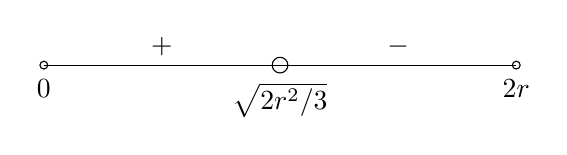
\begin{tikzpicture}	
		\draw
		(0,0) node[circle,draw,inner sep=1pt,label=below:$0$](){}
	-- (3,0) node[circle,draw,inner sep=2pt,label=below:$\sqrt{2r^2/3}$](){} node[midway,above]{$+$}
	-- (6,0) node[circle,draw,inner sep=1pt,label=below:$2r$](){} node[midway,above]{$-$};
	\end{tikzpicture}
\end{center}
Because $f'(c)>0$ for all $c\in(0,\sqrt{2r^2/3})$ and $f'(c)<0$ for all $c\in(\sqrt{2r^2/3},2r)$, the absolute maximum of $f$ must be at $x=\sqrt{2r^2/3}$.
\begin{align*}
	f\paren{\sqrt{\frac{2r^2}{3}}}
	&=2\pi\paren{\sqrt{\frac{2r^2}{3}}}^2\sqrt{r^2-\paren{\sqrt{\frac{2r^2}{3}}}^2}
	=2\pi\paren{\frac{2r^2}{3}}\sqrt{r^2-\frac{2r^2}{3}}
	=\frac{4\pi r^2}{3}\sqrt{\frac{r^2}{3}} \\
	&=\frac{4\pi r^2}{3}\cdot\frac{r}{\sqrt{3}}\cdot\frac{\sqrt{3}}{\sqrt{3}}
	=\boxed{\frac{4\pi\sqrt{3}r^3}{9}}
\end{align*}

\problem{12}
Use the same variables and notation as before. The only difference is a different definition of $f$.
\begin{align*}
	f(x)&=2\pi x^2+2\pi xh \\
	&=2\pi x^2+4\pi x\sqrt{r^2-x^2}
\end{align*}
\begin{align*}
	f'(x)=4\pi x+4\pi\sqrt{r^2-x^2}+4\pi x\cdot\frac{1}{2\sqrt{r^2-x^2}}\cdot(-2x)&=0 \\
	4\pi x+4\pi\sqrt{r^2-x^2}-\frac{8\pi x^2}{2\sqrt{r^2-x^2}}&=0 \\
	\frac{r^2-x^2}{\sqrt{r^2-x^2}}-\frac{x^2}{\sqrt{r^2-x^2}}&=-x \\
	r^2-2x^2&=-x\sqrt{r^2-x^2} \\
	r^4-4r^2x^2+4x^4&=x^2\paren{r^2-x^2} \\
	r^4-4r^2x^2+4x^4&=x^2r^2-x^4 \\
	5x^4-5r^2x^2+r^4&=0 \\
	x^2&=\frac{5r^2\pm\sqrt{25r^4-20r^4}}{10} \\
	x^2&=\frac{5r^2\pm\abs{r^2}\sqrt{5}}{10} \\
	x&=\pm\sqrt{\frac{5r^2\pm r^2\sqrt{5}}{10}} \\
	x&=\sqrt{\frac{5r^2\pm r^2\sqrt{5}}{10}}
\end{align*}
According to my calculator, $x=\sqrt{\dfrac{5r^2+r^2\sqrt{5}}{10}}$
is valid solution but $x=\sqrt{\dfrac{5r^2-r^2\sqrt{5}}{10}}$ is not.
\begin{center}
	\begin{tikzpicture}	
		\draw
		(0,0) node[circle,draw,inner sep=1pt,label=below:$0$](){}
	-- (5,0) node[circle,draw,inner sep=2pt,label=below:$\sqrt{\paren{5r^2-r^2\sqrt{5}/10}}$](){} node[midway,above]{$+$}
	-- (10,0) node[circle,draw,inner sep=1pt,label=below:$2r$](){} node[midway,above]{$-$};
	\end{tikzpicture}
\end{center}
Because $f'(c)>0$ for all $c\in\paren{0,\sqrt{\paren{5r^2-r^2\sqrt{5}/10}}}$ and $f'(c)<0$ for all $c\in\paren{\sqrt{\paren{5r^2-r^2\sqrt{5}/10}},2r}$, the absolute maximum of $f$ must be at $x=\sqrt{\paren{5r^2-r^2\sqrt{5}/10}}$.
\begin{align*}
	f\paren{\sqrt{\frac{5r^2+r^2\sqrt{5}}{10}}}
	&=2\pi\paren{\sqrt{\frac{5r^2+r^2\sqrt{5}}{10}}}^2+4\pi\paren{\sqrt{\frac{5r^2+r^2\sqrt{5}}{10}}}\sqrt{r^2-\paren{\sqrt{\frac{5r^2+r^2\sqrt{5}}{10}}}^2} \\
	&=2\pi\cdot\frac{5r^2+r^2\sqrt{5}}{10}+4\pi\paren{\sqrt{\frac{5r^2+r^2\sqrt{5}}{10}}}\sqrt{r^2-\frac{5r^2+r^2\sqrt{5}}{10}} \\
	&=2\pi\paren{\frac{5r^2+r^2\sqrt{5}}{10}+2\sqrt{\frac{5r^2+r^2\sqrt{5}}{10}}\sqrt{\frac{5r^2-r^2\sqrt{5}}{10}}} \\
	&=2\pi\paren{\frac{5r^2+r^2\sqrt{5}}{10}+2\sqrt{\frac{25r^4-5r^4}{100}}} \\
	&=2\pi\paren{\frac{5r^2+r^2\sqrt{5}}{10}+\frac{2\sqrt{20r^4}}{10}} \\
	&=2\pi\paren{\frac{5r^2+r^2\sqrt{5}+4\abs{r^2}\sqrt{5}}{10}} \\
	&=2\pi\paren{\frac{5r^2+5r^2\sqrt{5}}{10}} \\
	&=10\pi r^2\paren{\frac{1+\sqrt{5}}{10}} \\
	&=\boxed{\pi r^2\paren{1+\sqrt{5}}} \\
	&=\pi r^2\paren{\frac{1+\sqrt{5}}{2}}\cdot2 \\
	&=\boxed{2\pi r^2\phi}
\end{align*}
(Golden ratio appears somehow -- nice!)

\problem{13}
\begin{itemize}
	\item[(a)]
	Let $s,t$ be the side lengths of the square and triangle, respectively.
	\begin{align*}
		4s+3t&=10 \\
		t&=\frac{10-4s}{3}
	\end{align*}
	Let $f(s)$ be the combined area of the square and triangle.
	\begin{align*}
		f(s)&=s^2+\frac{\sqrt3}{4}\cdot t^2 \\
		&=s^2+\frac{\sqrt3}{4}\cdot\paren{\frac{10-4s}{3}}^2
	\end{align*}
	\begin{align*}
		f'(s)=2s+\frac{\sqrt3}{4}\cdot\Deriv[s]{\paren{\frac{10-4s}{3}}^2}&=0 \\
		2s+\frac{\sqrt3}{4}\paren{2\paren{\frac{10-4s}{3}}\paren{-\frac43}}&=0 \\
		2s-\frac{4\sqrt3\paren{10-4s}}{12}&=0 \\
		24s&=40\sqrt{3}-16\sqrt{3}s \\
		\paren{12+8\sqrt{3}}s&=20\sqrt{3} \\
		s&=\frac{20\sqrt3}{12+8\sqrt3} \\
		s&=\frac{5\sqrt3}{3+2\sqrt3}\cdot\frac{3-2\sqrt3}{3-2\sqrt3} \\
		s&=\frac{15\sqrt{5}-30}{9-12} \\
		s&=-\frac{3\paren{5\sqrt3-10}}{3} \\
		s&=-\paren{5\sqrt3-10} \\
		s&=10-5\sqrt3
	\end{align*}

	\item[(b)]
\end{itemize}

\end{document}
